\documentclass[11pt,a4paper]{article}
% ============================================================
% Shared preamble for Claude Experiments reports (pdflatex)
% Include this AFTER \documentclass in each report:
%   \documentclass[11pt,a4paper]{article}
%   % ============================================================
% Shared preamble for Claude Experiments reports (pdflatex)
% Include this AFTER \documentclass in each report:
%   \documentclass[11pt,a4paper]{article}
%   % ============================================================
% Shared preamble for Claude Experiments reports (pdflatex)
% Include this AFTER \documentclass in each report:
%   \documentclass[11pt,a4paper]{article}
%   \input{../preamble}
% ============================================================
\usepackage[T1]{fontenc}
\usepackage[utf8]{inputenc}
\usepackage[english]{babel}
\usepackage[a4paper,top=2.5cm,bottom=2.5cm,left=2.5cm,right=2.5cm]{geometry}
\usepackage{amsmath,amssymb}
\usepackage{graphicx}
\usepackage{subcaption}
\usepackage{booktabs}
\usepackage{xcolor}
\usepackage[colorlinks=true,allcolors=blue]{hyperref}
\usepackage{microtype}
\usepackage{float}
\usepackage{array}
\microtypesetup{expansion=false}

% Color scheme
\definecolor{colMicro}{HTML}{222222}
\definecolor{colExact}{HTML}{2878b5}
\definecolor{colPlacement}{HTML}{e07a1f}
\definecolor{colBoundary}{HTML}{429c74}
\definecolor{colCurrent}{HTML}{c23b55}
\definecolor{colMM}{HTML}{c23b55}

\providecommand{\SIG}{\textcolor{green!50!black}{\textbf{*}}}
\providecommand{\NS}{\textcolor{gray}{n.s.}}
\providecommand{\DRMS}{\Delta\mathrm{RMST}}
\providecommand{\ci}[2]{$[{#1},\;{#2}]$}

% ============================================================
\usepackage[T1]{fontenc}
\usepackage[utf8]{inputenc}
\usepackage[english]{babel}
\usepackage[a4paper,top=2.5cm,bottom=2.5cm,left=2.5cm,right=2.5cm]{geometry}
\usepackage{amsmath,amssymb}
\usepackage{graphicx}
\usepackage{subcaption}
\usepackage{booktabs}
\usepackage{xcolor}
\usepackage[colorlinks=true,allcolors=blue]{hyperref}
\usepackage{microtype}
\usepackage{float}
\usepackage{array}
\microtypesetup{expansion=false}

% Color scheme
\definecolor{colMicro}{HTML}{222222}
\definecolor{colExact}{HTML}{2878b5}
\definecolor{colPlacement}{HTML}{e07a1f}
\definecolor{colBoundary}{HTML}{429c74}
\definecolor{colCurrent}{HTML}{c23b55}
\definecolor{colMM}{HTML}{c23b55}

\providecommand{\SIG}{\textcolor{green!50!black}{\textbf{*}}}
\providecommand{\NS}{\textcolor{gray}{n.s.}}
\providecommand{\DRMS}{\Delta\mathrm{RMST}}
\providecommand{\ci}[2]{$[{#1},\;{#2}]$}

% ============================================================
\usepackage[T1]{fontenc}
\usepackage[utf8]{inputenc}
\usepackage[english]{babel}
\usepackage[a4paper,top=2.5cm,bottom=2.5cm,left=2.5cm,right=2.5cm]{geometry}
\usepackage{amsmath,amssymb}
\usepackage{graphicx}
\usepackage{subcaption}
\usepackage{booktabs}
\usepackage{xcolor}
\usepackage[colorlinks=true,allcolors=blue]{hyperref}
\usepackage{microtype}
\usepackage{float}
\usepackage{array}
\microtypesetup{expansion=false}

% Color scheme
\definecolor{colMicro}{HTML}{222222}
\definecolor{colExact}{HTML}{2878b5}
\definecolor{colPlacement}{HTML}{e07a1f}
\definecolor{colBoundary}{HTML}{429c74}
\definecolor{colCurrent}{HTML}{c23b55}
\definecolor{colMM}{HTML}{c23b55}

\providecommand{\SIG}{\textcolor{green!50!black}{\textbf{*}}}
\providecommand{\NS}{\textcolor{gray}{n.s.}}
\providecommand{\DRMS}{\Delta\mathrm{RMST}}
\providecommand{\ci}[2]{$[{#1},\;{#2}]$}

\title{CE-09: Boundary Placement Diagnostic}
\author{Two-Layer CTMC Experiments Pipeline}
\date{August 4, 2026}
\begin{document}\maketitle
\begin{abstract}
CE-09 compares uniform placement, static boundary-weighted placement, and an oracle exact/exact mode across six sparse regimes. The results do not support static boundary placement as a generally reliable correction: it reduced absolute normalized RMST error in only one of six cells and sometimes changed premature bias into late bias. The oracle mode remained close to Full Micro, confirming that dynamic active-edge information is valuable. However, the current design is not a clean causal placement ablation because placement modes use different network seed blocks and the oracle also changes the hazard.
\end{abstract}
\section{Design audit}
Each row contains 40 paired comparisons of one experimental mode against a Full Micro reference on the same network. Across placement modes, however, the runner increments \texttt{base\_seed} by cell, so uniform, boundary, and oracle modes do not share networks replication-by-replication. In addition, \texttt{oracle\_exact} invokes exact active-edge hazard plus exact placement, not aggregate hazard plus exact placement. Consequently, within-row variant-vs-Micro estimates are valid, but differences between modes are unpaired ensemble diagnostics, not isolated causal placement effects.

\section{Results}
\begin{table}[H]\centering
\caption{$\Delta$RMST/$T_{end}$ by regime and mode.}
\begin{tabular}{rrrrr}\toprule
$d$ & $k$ & Uniform & Boundary & Exact/exact oracle\\\midrule
4&2&-0.1093&-0.0635& 0.0148\\
4&5&-0.0490&-0.0602& 0.0043\\
6&2&-0.0416&-0.0523&-0.0253\\
6&5&-0.0335&-0.0338&-0.0078\\
12&2&-0.0284& 0.0360&-0.0006\\
12&5&-0.0041& 0.0096& 0.0068\\
\bottomrule\end{tabular}
\end{table}
All modes completed all runs. Static boundary placement improved absolute normalized RMST only for $(d,k)=(4,2)$; it was neutral or worse elsewhere and overshot to positive error in both $d=12$ cells. The exact/exact oracle was near zero in five cells and modestly premature in $(6,2)$.
\begin{figure}[H]\centering
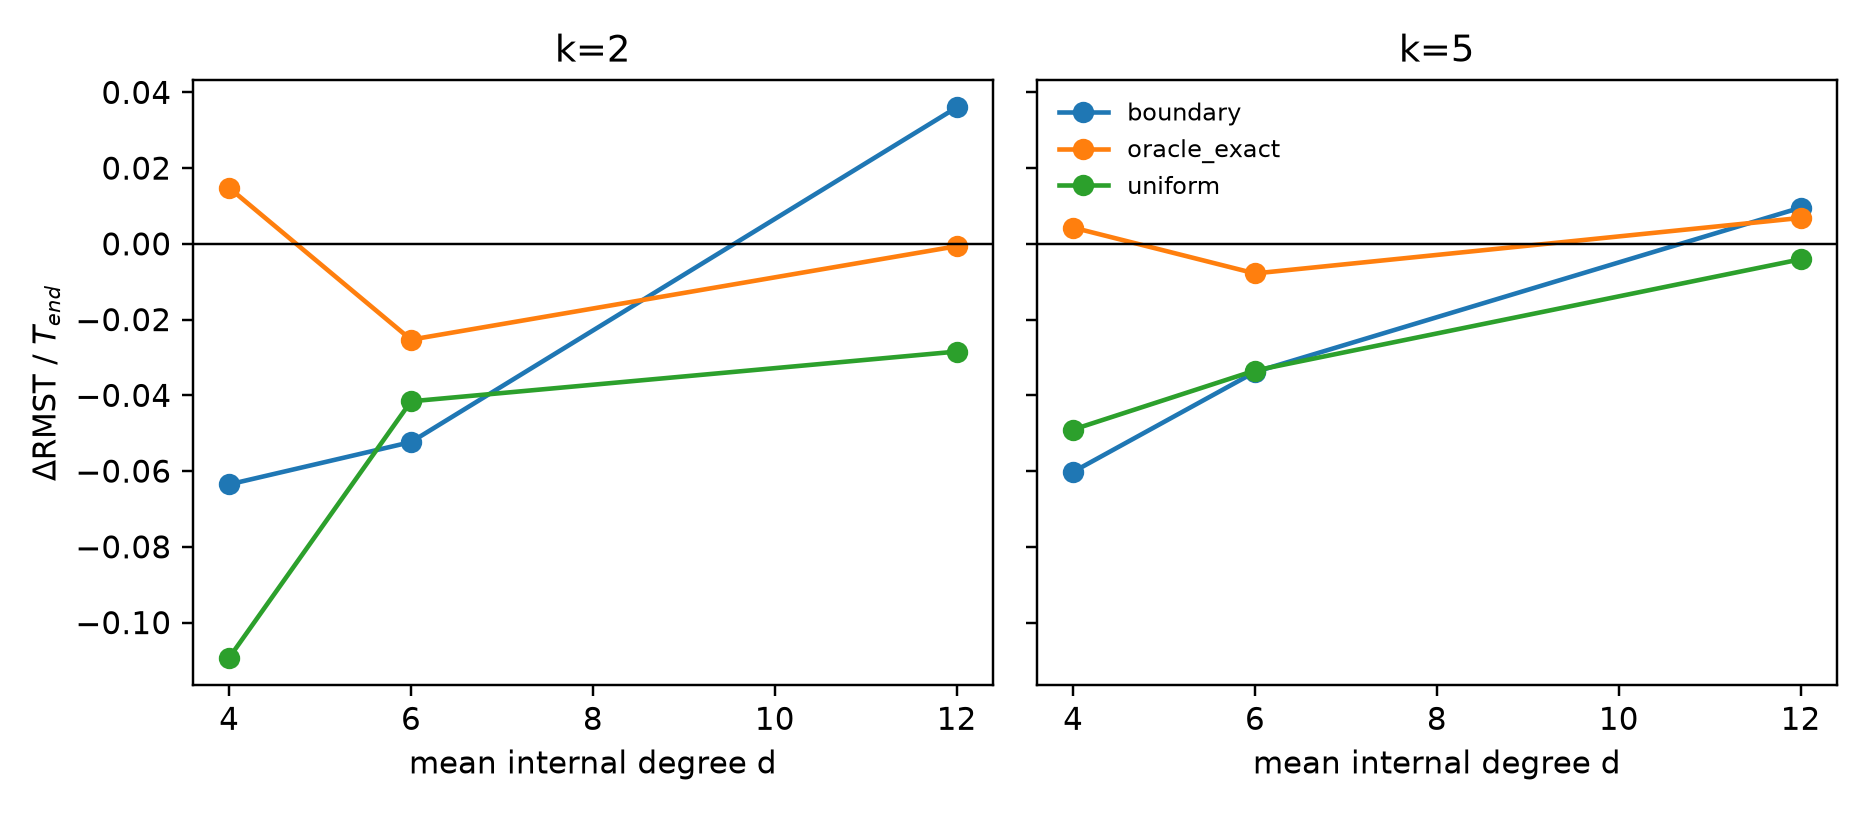
\includegraphics[width=.9\linewidth]{figures/placement_diagnostics.png}
\caption{Variant-vs-own-Micro diagnostics. Lines must not be read as paired placement contrasts.}
\end{figure}

\section{Implications}
Knowing only that a node lies on a static boundary is insufficient. Boundary nodes can be reached early or late depending on their internal degree, distance from the imported seed, and currently infected source endpoints. A static boundary rule may place infection at a gateway too aggressively, explaining the late-sign overshoot after it changes subsequent propagation paths.

For error reduction, boundary descriptors should gate a rate correction rather than directly force placement, or placement should use a parameters-only degree distribution with an explicit dense-community self-disable. Before using CE-09 for causal attribution, a corrected CE-09b must share network and initialization seeds across all modes and compare only mathematically defined cells. Aggregate-hazard/exact-placement remains undefined when aggregate hazard is positive but no active edge exists.
\section*{Reproduction}
\texttt{.venv/bin/python extrascripts/run\_ce09\_boundary\_isolation.py --grid full --workers 12 --resume}
\end{document}
